\documentclass{article}
\usepackage[utf8]{inputenc}
\title{Lecture 2; relational databases}
\author{wbg231 }
\date{December 2022}
\newcommand{\R}{$\mathbb{R}$}
\newcommand{\B}{$\beta$}
\newcommand{\A}{$\alpha$}
\newcommand{\D}{\Delta}

\newcommand{\avector}[2]{(#1_2,\ldots,#1_{#2})}
\newcommand{\makedef}[2]{$\textbf{#1}$:#2 }
\usepackage{tikz,graphicx,hyperref,amsmath,amsfonts,amscd,amssymb,bm,cite,epsfig,epsf,url}

\begin{document}

\maketitle

\section{introduction}
\begin{itemize}
\item \href{https://brightspace.nyu.edu/d2l/le/lessons/261985/topics/8323144}{slide link}
\item data base management systems and structured query language (SQL) are form the 70's 
\item despite this they have not gone our of vague 
\item prior to the 70's data base management was done with file systems 
\item there are a few limitations to using file systems for data base management 
\begin{itemize}
    \item there are no constraints on data formats or validation 
    \item they do not support content based queries 
    \item there is no protocol for concurrent access (ie what happens if two people modify a data base at the same time) 
\end{itemize}
\section{data base management systems (DBMS)}
\item DBMS's job is to provide the following
\begin{itemize}
    \item data integrity/ consistency
    \item concurrent access
    \item standardized formatting 
    \item standardized query interface or language 
\end{itemize}
\item there are many types of DBMS but we are going to focusing today on relational data base management systems 
\section{the relational model}
\item at a high level tables of data
\item each column represents a set of possible values
\item a relation over sets $A_1...A_n$ is a subset of their Cartesian  product 
\begin{itemize}
    \item $R\subseteq A_1\times A_2...\tiems A_N$
    \item the rows are the table are elements of R also known as tuples
    \item $(a_1..a_n)\in R\Rightarrow a_1\in A_1...a_n\in A_n$
\end{itemize}
\subsection{example}
\item consider the relation pachyderms 
\item $A_1=\{s|s \text{is a string}\}$ species 
\item $A_2$ era is a list of era names that must come from a pre set list of values 
\item $a_3$ is a list of diets that also must come from a pre set list of values representing the diet
\item $a_4$ is a Boolean representing extent 
\item any column could take on either a finite or infinite set of values 
$R\subset A_1\times A_2\times A_3\times a_4$ does not have to contain all combinations 
\item 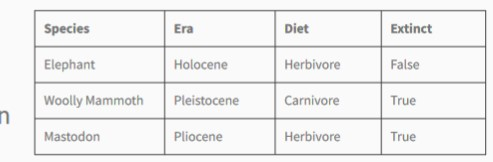
\includegraphics[width=5cm]{lecture notes/week 2/immages/w_1_1.jpg}
\subsection{relation vs tables}
\item relations are the abstract model of data 
\tiem tables refer to an explicitly constructed relation 
\item other relations in database 
\begin{itemize}
    \item view:  a relation defined implicitly and constructed dynamically at run time 
    \itme a temporary table the output of a query
\end{itemize}
\subsection{properties of a relation}
\item the Cartesian product $R\subseteq A_!\times A_2\tiems A_3\times A_4$ is a set 
\begin{itemize}
    \item the tuples in R are under 
    \item the tuples are unique ie there are no duplicate rows
    \item relations over common domains columns can be combined by set operations
\end{itemize}
\item in practice add a column with identifiers to force uniqueness
\begin{itemize}
    \item this identifier is not usually part of the data but generated by the data base management system 
    \item ID fields are often used as primary keys and give a default order to rows
\end{itemize}
\subsection{slido example}
\item if A has 5 elements B has 3 elements and $A\cap B= \emptyset$ how many possible relations exist using A and B
\item solution 
\begin{itemize}
    \item we know that $|A|=5, |B|=3$ thus $|A\times B|=15$
    \item note that the question does not pose an order for A,B so order matters
    \item we know $R \subseteq |A\times B|\cup |B\times A|$ thus $R\in P(A\times B)\cup P(B\times A)$ where p represents the power set 
    \item $|P(A\times B)|=2^|A\times B|=2^{15}=P(B\times A)$
    \item not here that $\emptyset \in P(A\times B)$ and  $\emptyset \in P(B\times A)$ 
    \item so to avoid double counting the total number of relations is $P(A\times B)+P(B\times A)-1=2^15+2^{15}-1=2^{16}-1$
\end{itemize}
\item 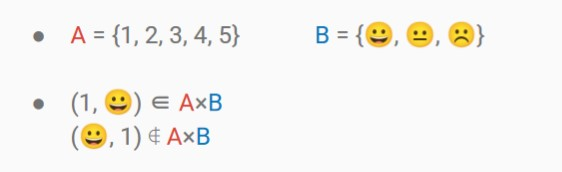
\includegraphics[width=5cm]{lecture notes/week 2/immages/w_1_2.jpg}
\item the order of the tuples matter
\section{Schemas}
\item a relation is defined by a Schema
\item for instance the Pachyderms relation has schema $Pachyderms(id:int, Species: string, era:string, Diet:string, extinct:boolean)$ this tells us that any tuple of the form $(int, string, string, boolean)$ is valid under this schema 
\item schema in force type not correctness
\subsection{sachems can be hard to design well}
\item imagine we want to make a schema to track customers
\item $customer(id :int, lastname:string, firstname:string)$
\item are all strings valid names?

\subsection{slido}
\item what constraints should you add to the name field of a customer database to ensure data integrity?
\item solution 
\begin{itemize}
    \item length constraints wont work, that could be discriminatory against one cloture or another
    \item so are character constraints, some people have special characters in there names
    \item it is difficult to query and link databases if the data must be modified to fit a schema 
    \item further constraints can have disproportionate effects on different sub populations 
    \item so in full there is no "correct" constraint
\end{itemize}
\section{relational database}
\item a relational database consists of one or more relational schema 
\item structured data can be encoded by joining on shared attributes
\item the collection of schema defines your data model 
\subsection{keys}
\item keys are what determine the identity of a row
\item key can be simple (over a single column) or compound (over multiple columns) 
\item you can have a primary and alternate keys (primary key is often numeric) 
\subsection{foreign keys}
\item a key from one relation can be a column or attribute in another (this is called a foreign key constraint) 
\item this can be used to ensure consistency between tables
\item this is not automatic you need to specify this during schema definition 
\item 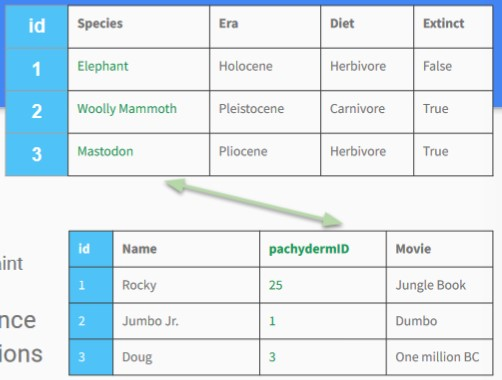
\includegraphics[width=5cm]{lecture notes/week 2/immages/w_1_3.jpg}
\subsection{normalization}
\item a database schema is normal if not redundantly stored. (that is we use identifiers not values to link between relations)
\item this makes modifying a record easy since that data exist only in one place
\item but this can be difficult or complex. 

\section{summary of relations}
\item we like relations 
\item they are used all over in the real world 
\item databases consist of far More than one relation 
\item putting data into a retinal model can make it easier to work with 
\item schema provide some degree of safety and data validation 
\section{SQL}
\item Structured Query Language (SQL)
\item SQL is the language we used to talk to databases. it is not a procedural language like Python or C, it is instead declarative
\item a declarative language   means you state what you want not the computation or algorithm to get it 
\item think of sql as more of a protocol than a programming language 
\item SQL is an ANSI standard but different implementations have different quirks
\subsection{selecting data }
\item example select query SELECT $A_1, A_2
FROM Relation
WHERE A_i > 2$ 
\item $*$ means all 
\item the result of a SELECT is always another relation
\item typically we iterate over rows produced by select in your host language: python example
\\ for row in db.execute(ʻSELECT * FROM Pachyderms):\\$\quad  print(row)$
\subsection{joining relations}
\item data is typically structured across multiple relations 
\itme we can combine relations using JOIN
\item outline of join types \\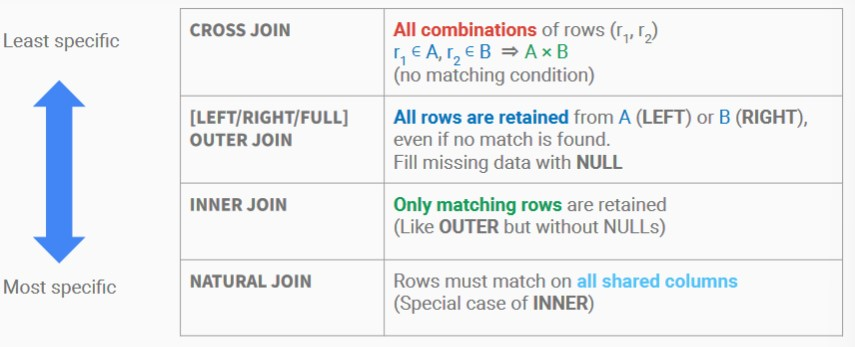
\includegraphics[width=10cm]{lecture notes/week 2/immages/w_1_4.jpg}
\item inner and outer joins are the most common types of joins
\subsection{modifying data}
\item INSERT INTO table (column1, column2, ...)
VALUES (value1, value2, ...),
[$(row_2_value1, row_2_value2, ...), ...]$
\item UPDATE table
SET column1 = value1, column2 = value2, ...
WHERE [some condition]

\subsection{SQL injection}
\item have to be care for SQL injection attacks 
\\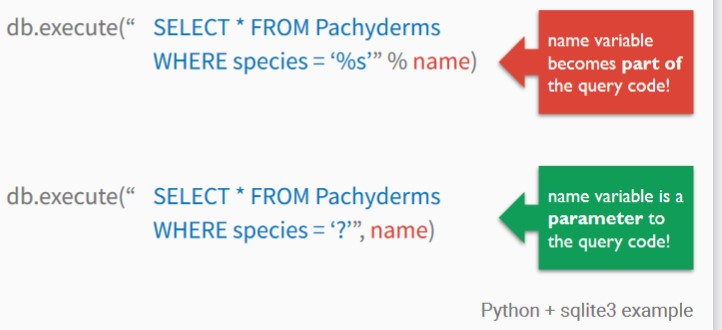
\includegraphics[width=10cm]{lecture notes/week 2/immages/w_1_5.jpg}
\item so we like the bottom one because it is passed as a parameter to the query code instead of part of query code. 

\section{Aggregation }
\subsection{ Aggregation  Queries}
\item Aggregation let us summarize multiple tuples in a single result 
\item example average height of people based on zip code : SELECT Zip, AVG(Height) FROM Residents GROUP BY Zip 
\subsection{useful aggregators}
\item AVG, SUM, MIN, MAX do what you would expect
\item COUNT(DISTINCT x) returns the number of unique values in column X
\item COUNT(*) number of rows, Count(X) number of non-null rows
\item $group_concat(x)$ concatenate string values
\item $group_concat(x,y)$ concatenate join(x,y)
\subsection{aggregation conditions}
\item SELECT ... WHERE [condition] GROUP BY [fields]
\item WHERE clause applied to inputs not outputs 
\item SELECT ... GROUP BY [fields] HAVING [condition]
\item HAVING applies to outputs
\section{indexing}
\subsection{logical and physical storage}
\item relational schemes hold the data as a set of tuples
\item this may not be the best way to organize the data internally
\begin{itemize}
    \item organizing by a column could be more efficient 
    \itme could also use specific data structures like has tables or trees
\end{itemize}
\item RDBMS abstract these decisions, but you can specifies them if you know how the data will be used
\subsection{indexing}
\item an index is a data structure over one or more columns that can accelerate queries.
\item example:
\begin{itemize}
    \item a table has a few distinct values that are repeated many times 
    \item frequently want all rows with one given value 
    \item it might be faster to store a mapping $values\rightarrow rows$ then to search each row independently
\end{itemize}
\subsection{draw backs of indexing}
\item constructing index takes time and space
\item the more complex the index the more costly
\item  updates become slower
\item there is no guarantee it will speed up queries
\subsection{when to index}
\item when data is read more often than written
\item when queries are predictable
\item when queries rely on a small number of attributes
\item remember indices can always be deleted
\section{data bases can ensure the integrity of transactions}
\subsection{file system draw back:consistency}
\item  file systems have a hard time imposing consistency on data
\item what if we want to impose constraints on our data 
\item example
\begin{itemize}
    \item guaranteeing the a graph is connected
    \item vertices stored in nodes.dat
    \item edges stores in edges.dat
    \item what if you want to add a vertex and two edges?
\end{itemize}
\item if you add a vertex first the graph becomes disconnected
\item if you add edges first those edges lead no where and are thus invalid 
\item either operation makes the data inconsistent 
\item thus operations need to be preformed simultaneously but file systems do not do this 
\item so we need another layer of abstraction 
\subsection{file system draw backs:concurrent access}
\item in a file system if two process are reading from a file at the same time we are fine 
\item if either is reading and  writing then there are consistency issues
\item this issue is called concurrent access, and file systems don't know how to deal with this 

\section{ACID}
\item ACID is an acronym describing good priorities of a DBMS
\begin{itemize}
    \item A (Atomicity)- operations are all or nothing (no partial updates, operations are bundled in transactions)
    \item C (Consistency): transactions only move from one valid state to another
    \item I (isolation): concurrent operations do not depend on order of execution 
    \item D (Durability): completed transactions are parameterise so they are written to disk after completed 
\end{itemize}
\subsection{Atomicity  in practice}
\item when modifying tables, wrap queried statements like this 
\begin{itemize}
    \item begin transaction;[queries]; COMMIT
    \item or 
    \item begin transaction;[queries]; ROLLBACK
\end{itemize}
\item that is if a query fails mid transaction uncommitted changes will be abandoned. this makes sure that the database is always in a valid state
\subsection{transaction example}
\item transactions are like try except blocks in Python
\item think of SQL interactions as a conversation each command executes and either succeeds or fails 
\item if you are preforming multiple queries and one of them fails, you roll back to the database state before any were run 
\item if all are run successfully you commit the transaction (that is all queries) 
\item example \\ 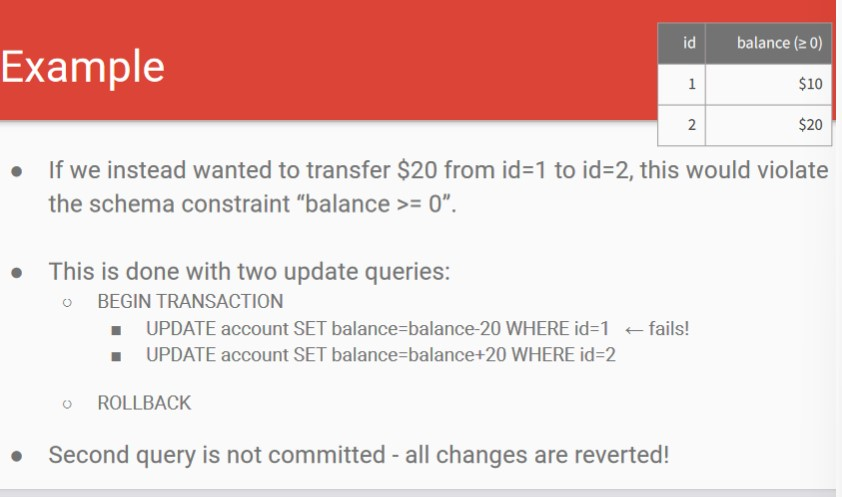
\includegraphics[width=10cm]{lecture notes/week 2/immages/w_1_6.jpg}

\subsection{consistency in practice}
\item consistency is maintained by the schema 
\item you can add a check to the schema like this CREATE TABLE Pachyderms ( id INTEGER PRIMARY KEY,
species TEXT NOT NULL,
height NUMBER CHECK (height >= 1.0))
\item then if the data fails that check the operations fails immediately meaning the data can not enter an invalid state
\subsection{Isolation in practice}
\item ussualy achived by locking the database during modification. that is only one transaction can modify the data at a time 
\item Thai becomes an issue for distributed databases like twitter
\item map reduce side steps this problem 
\subsection{git}
\item git can be seen as a kind of distributed non relational data base 
\iteim it is acid \\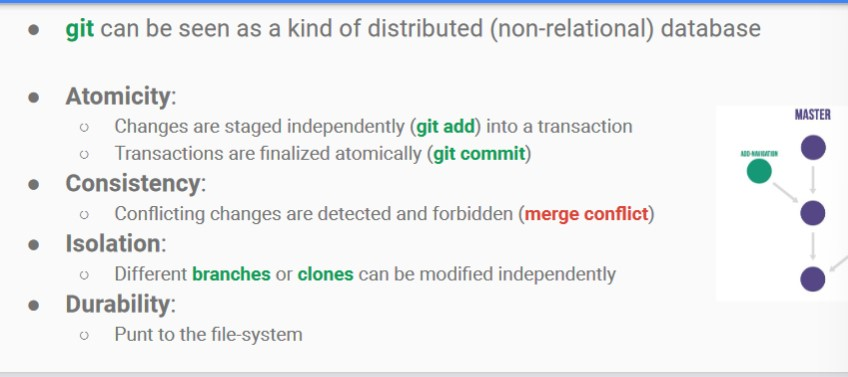
\includegraphics[width=10cm]{lecture notes/week 2/immages/w_1_7.jpg}
\subsection{slido}
\item which property would most fix the connected graph problem discussed above?
\item they did not give us the solution to this, i think it would atomicity (you can bundle add edges and vertices as a transaction and if all are completed then we are good)




\end{itemize}

\end{document}
